%% Copyright 1998 Pepe Kubon
%%
%% `two.tex' --- 2nd chapter for thes-full.tex, thes-short-tex from
%%               the `csthesis' bundle
%%
%% You are allowed to distribute this file together with all files
%% mentioned in READ.ME.
%%
%% You are not allowed to modify its contents.
%%

%%%%%%%%%%%%%%%%%%%%%%%%%%%%%%%%%%%%%%%%%%%%%%%%%
%
%     Chapter 6  
%
%%%%%%%%%%%%%%%%%%%%%%%%%%%%%%%%%%%%%%%%%%%%%%%%

\chapter{Experiments}
\label{ch:exp}

In this chapter, we will evaluate our approach by reporting the experimental results with respect to the running time on computing the subspace skyline on both real data sets and synthetic data sets. We compare the running time of the algorithms with and without using pruning method. Both of the algorithms compute the subspace skyline using \emph{dominating candidate sets} enumeration framework. The only difference between these two algorithms we compare is whether the pruning method is applied.

We implement our algorithms using C++. We use Microsoft Visual Studio 2010 to compile our C++ programs. Experiments were conducted on a PC with an Intel Core(TM) i7-3779 3.40GHz CPU, 16GB main memory and a 900G hard disk, running the Microsoft Windows 7 Enterprise Edition operating system.

\section{Experiments of Skyline Subspace Query on Graph}
\label{ch:exp:graph}
In this section, we will introduce the empirical study on skyline subspace queries on graphs. In all of the experiments of this section, we uniformly choose 100 nodes as the query nodes and compute the average running time of those queries.
Using the model of Kronecker graph provided by~\cite{leskovec2005realistic}, we generated graphs of different sizes.
According to~\cite{leskovec2005realistic}, a Kronecker graph has several real world network properties:
heavy tails for the in-degree and out-degree distributions;
heavy tails for the eigenvalues and eigenvectors;
small diameters; and the ``Densification Power Law" (DPL).

We use the MATLAB code from graph500 \footnote{\url{http://www.graph500.org/specifications\#sec-3_3}} to generate graphs with scale from $15$ to $20$ which corresponds to the number of vertices from $2^{15}$ to $2^{20}$. All the graphs with different sizes are generated from the initial matrix:
\begin{equation}
\begin{bmatrix}
0.3 & 0.24\\ 
0.24 & 0.22
\end{bmatrix}
\end{equation}

with edge factor $2$ which is the expected average degree of the vertices. The label is generated in Pareto distribution which is a Power Law Distribution. We use the Pareto function from a python package numpy \footnote{\url{http://docs.scipy.org/doc/numpy/reference/generated/numpy.random.pareto.html}} to generate the label information of the vertices. We randomly generate 1000 different labels for these graphs in power law distribution. Our algorithms run skyline subspace queries in $2$-hops neighbourhood. Figure~\ref{fig:exp:kronecker} shows that the speed-up factor of algorithm with pruning is increasing with increasing number of labels. Neither method is linearly scalable with respect to the number of the labels.

\begin{figure}[h]
    \centering
      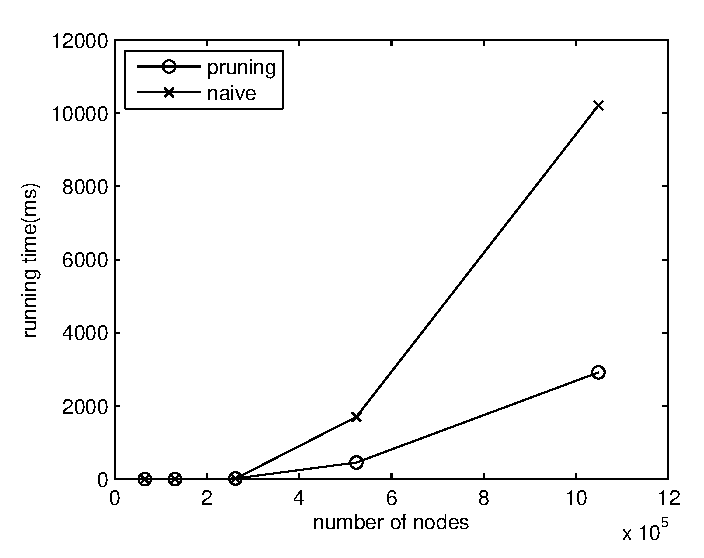
\includegraphics[width=0.7\textwidth]{figs/kronecker}
    \caption{Kronecker graph with 1000 different labels}
    \label{fig:exp:kronecker}
\end{figure}

\begin{table}[h]
    \centering
    \begin{tabular}{|l|l|l|}
    \hline
    datasets                   & Facebook Network & DBLP Network \\ \hline
    number of nodes            & 4039             & 906505       \\ \hline
    number of edges            & 88234            & 1656732      \\ \hline
    number of different labels & 20               & 1000         \\ \hline
    average degree             & 21.8455          & 1.8276       \\ \hline
    \end{tabular}
    \label{tab:exp:fb_dblp}
    \caption{Dataset statistics}
\end{table}

We also do some empirical study on real world datasets. We download a dataset of Facebook network from \emph{Stanford Network Analysis Project} \footnote{\url{http://snap.stanford.edu/data/egonets-Facebook.html}}. In Figure~\ref{fig:exp:fb}, we show the running time of our algorithms in 4-hops neighbourhood with different numbers of unique labels in total. The labels are assigned to the vertices in uniform distribution. In the Facebook network dataset, the running time of the algorithm with pruning is much less than the running time of the algorithm without pruning. We note that neither method is linearly scalable with respect to the size of the graphs. 

\begin{figure}[h]
    \centering
      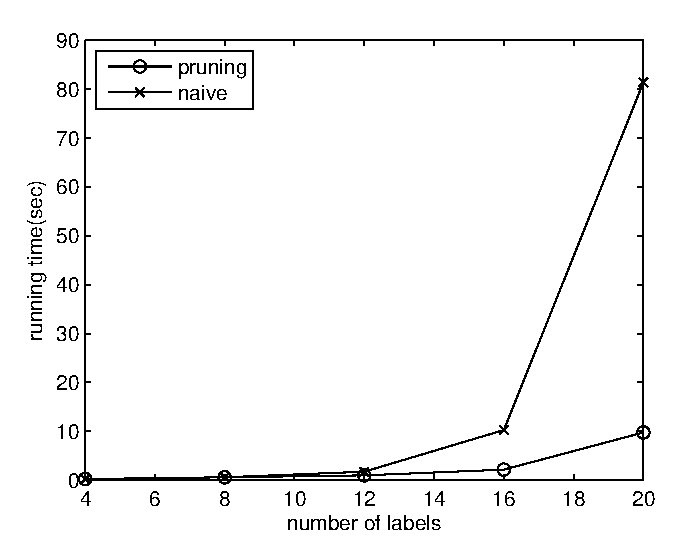
\includegraphics[width=0.7\textwidth]{figs/FB}
    \caption{Running time of the algorithms on facebook network}
    \label{fig:exp:fb}
\end{figure}

Figure~\ref{fig:exp:fb_dis} shows the distribution of the labels in the Facebook network dataset. The of degrees of most of the vertices are less than 200 while some of the vertices are with degrees greater than 800.

\begin{figure}[H]
    \centering
      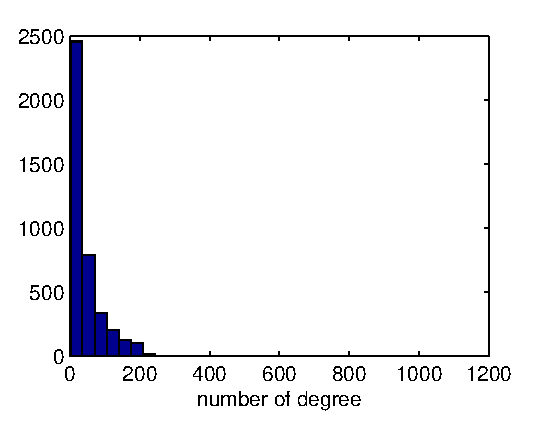
\includegraphics[width=0.5\textwidth]{figs/fb_distri}
    \caption{Facebook network degree distribution}
    \label{fig:exp:fb_dis}
\end{figure}

Figure~\ref{fig:exp:fb_hops} shows the running time of our algorithms with 20 unique labels in different numbers of hops. The speed-up factor of the pruning-based algorithm is increasing with the number of hops.

\begin{figure}[H]
    \centering
      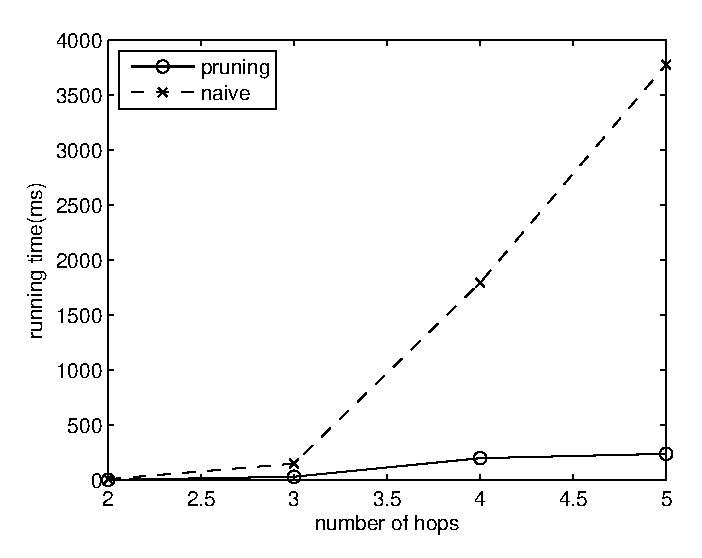
\includegraphics[width=0.5\textwidth]{figs/FB_hops}
    \caption{Running time of the algorithms with different numbers of hops}
    \label{fig:exp:fb_hops}
\end{figure}


We also use the DBLP dataset from $arnetminer$ \footnote{\url{http://arnetminer.org/billboard/citation}} to evaluate the performance of our algorithms. The DBLP dataset provides us the author list of each publication. We build a citation network based on these author lists in the following way. We add an edge between author $X$ and author $Y$ if and only if $X$ is one of the top ten co-authors of $Y$ and $Y$ is one of the top ten co-authors of $X$. We choose the top one thousand most frequent conferences as the labels of the vertices. If an author publishes more than five papers in a conference, then we add the corresponding label of that conference to that vertices. Figure~\ref{fig:exp:dblp} shows that the pruning-based algorithm is about 10 times faster than the algorithm without pruning on DBLP network. We note that neither algorithm is linearly scalable with respect to the size of the graphs.

\begin{figure}[H]
    \centering
      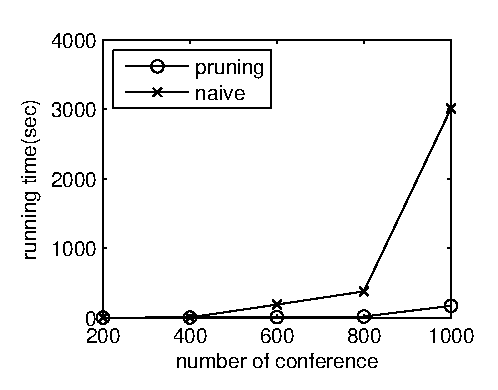
\includegraphics[width=0.7\textwidth]{figs/DBLP}
    \caption{Running time of the algorithms on DBLP network}
    \label{fig:exp:dblp}
\end{figure}

Figure~\ref{fig:exp:dblp_dis} shows the distribution of the degrees of the DBLP network. Comparing to the facebook network, the variance of the degrees of the vertices is not very large.

\begin{figure}[H]
    \centering
      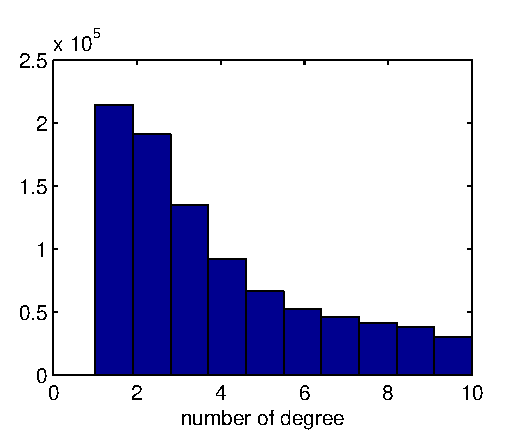
\includegraphics[width=0.5\textwidth]{figs/DBLP_distri}
    \caption{DBLP network degree distribution}
    \label{fig:exp:dblp_dis}
\end{figure}

\section{Experiments of Spatial Skyline Subspace Query}
\label{ch:exp:spatial}
In this section, we will introduce the empirical study on spatial skyline subspace query. We use the Yelp Academic Dataset \footnote{\url{https://www.yelp.ca/academic_dataset}} to evaluate our algorithms. Yelp Academic Dataset provides 13490 different business spots. Each business spot consists of its longitude and latitude information. We use the longitude and latitude information of the business spot as its $XY$ spatial information. The business spot consists of a set of category information, neighbourhood information and university information. We use those information as the labels of the business spot. Each business spot also contains a stars rating.

In Figure~\ref{fig:exp:yelp20l}, we choose the top 20 most popular categories as the labels of the business spot and we compare the running time of the algorithms in the sense of different radii. The running time of the prune-based algorithm is about 2 times faster than the algorithm without pruning.

\begin{figure}[h]
    \centering
      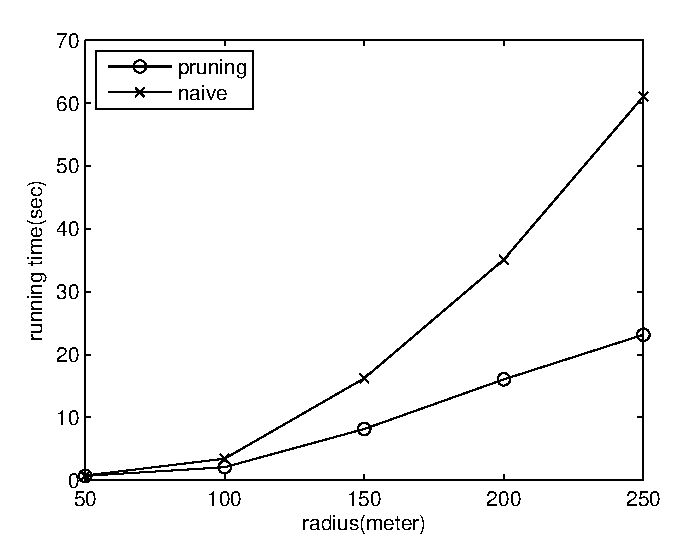
\includegraphics[width=0.7\textwidth]{figs/YelpTop20Labels}
    \caption{Yelp Data Set with Top 20 most popular categories}
    \label{fig:exp:yelp20l}
\end{figure}

In Figure~\ref{fig:exp:yelp300l}, we choose the top $300$ most popular categories as the labels of the business spot. We assign a category to a business spot as a label if the business has the highest star rating among all the business with that category. We note that both algorithms are linearly scalable with respect to radius. Table~\ref{tab:exp:radius} shows the average number of business spots in terms of radius in yelp dataset.

\begin{figure}[h]
    \centering
      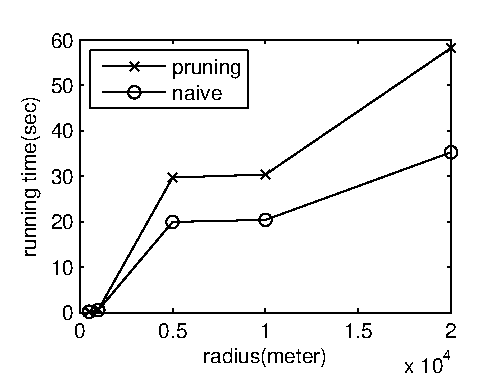
\includegraphics[width=0.7\textwidth]{figs/Yelp300Labels}
    \caption{Yelp Data Set with 300 different labels}
    \label{fig:exp:yelp300l}
\end{figure}


\begin{table}[h]
\centering
\begin{tabular}{|l|l|}
\hline
Radius (meters) & Number of Points \\ \hline
50              & 11               \\ \hline
100             & 26               \\ \hline
150             & 42               \\ \hline
200             & 59               \\ \hline
250             & 76               \\ \hline
500             & 159              \\ \hline
1000            & 298              \\ \hline
5000            & 597              \\ \hline
10000           & 657              \\ \hline
20000           & 721              \\ \hline
\end{tabular}
\caption{Number of points in certain radii in average.}
\label{tab:exp:radius}
\end{table}

We also evaluate the running time of the algorithm on data with the radius fixed but the number of labels is different. In this thesis, we conduct the empirical study on the large neighbourhood queries whose label collection radius is 10000 meters. we first get a random permutation of the labels. Second, we run our programs on the first $100$ labels, the first $200$ labels, $\dots$, etc. Figure~\ref{fig:exp:yelp10k} shows the running time per query in average. The running time of the pruning-based algorithm does not have significant better performance than the algorithm without pruning.

\begin{figure}[h]
    \centering
      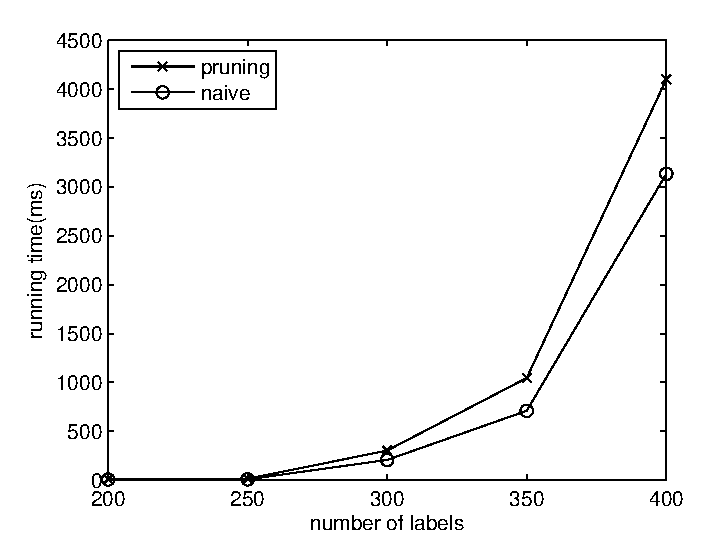
\includegraphics[width=0.7\textwidth]{figs/Yelp10Kmeters}
    \caption{Yelp Data Set in 10000 meters neighbourhood}
    \label{fig:exp:yelp10k}
\end{figure}

Figure~\ref{fig:exp:spatial} shows the running time of spatial synthetic data with 20 different labels. Both the spatial points and the labels of the points are generated randomly in uniform distribution. The pruning-based algorithm is 7 times faster than the naive algorithm when the radius is 40000.

\begin{figure}[h]
    \centering
        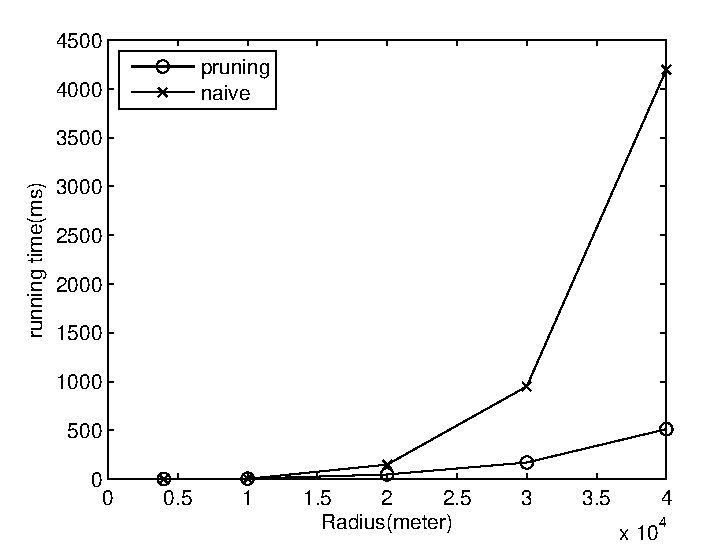
\includegraphics[width=0.7\textwidth]{figs/Spatial}
    \caption{Spatial Synthetic Dataset}
    \label{fig:exp:spatial}
\end{figure}

In summary, the experimental result shows that our algorithms compute the skyline subspace efficiently and the pruning methods improve the running time of the programs effectively.